\documentclass[runningheads]{llncs}

%%%%%%%%%%%%%%%%%%%% Non standard in llncs %%%%%%%%%%%%%
\usepackage[top=1.5in, bottom=1.5in, left=1.5in, right=1.5in]{geometry}


%\usepackage{appendix}
\usepackage{chngpage}
% Allows Diagram Sketching
%
\usepackage[all]{xy}
\usepackage{tikz}
%
% Comments
%
\usepackage{comment}

%
% Math symbols
%
\usepackage{amssymb}
\usepackage{amsmath}
\usepackage{amsthm}
%\newtheorem{theorem}{Theorem}
%
% Figures
%
\usepackage{wrapfig}
\usepackage{float}
\floatstyle{boxed}
\restylefloat{figure}
\usepackage{graphicx}
\usepackage{indentfirst}
%
% Algorithmic code
%
\usepackage{algorithmic}
\usepackage{algorithm}
\usepackage{listings}

\usepackage{hyperref}
\usepackage{cite}
\usepackage{enumitem}
\setlist{nosep}


\lstset{
captionpos=b, 
frame=bt,
basicstyle=\footnotesize,
tabsize=4,
morekeywords={split,join, drop,Bit,random}, 
keywordstyle=\color{blue},
breaklines=true}


%
% Colours to the revision process
%
\usepackage{color}
\definecolor{blue}{rgb}{0,0,1}
\definecolor{red}{rgb}{1,0,0}
\definecolor{black}{rgb}{0,0,0}



%Hyperlinks
%
\usepackage{hyperref}

%
% Local macros
%
\def\equiv{\Leftrightarrow}
\def\conv#1{#1^\circ}
\def\comp{\mathbin{\cdot}}
\def\just#1#2{\\ &#1& \rule{2em}{0pt} \{ \mbox{\rule[-.7em]{0pt}{1.8em} \small #2 \/} \} \nonumber\\ && }
\def\quotes#1{``#1''}
% -- to dos
\newcount\td \td=0 %  to-do counter
\long\def\Todo#1{\vskip 1ex\noindent\fcolorbox{red!60}{white!20}{
\global\advance\td by 1
\textbf{To-do (\number\td):}\\~
\begin{minipage}{.75\textwidth}
#1
\end{minipage}
}\vskip 1ex}
% ----- shorthands ----
\def\eqref#1{(\ref{#1})}

%Revised
%
 
\long\def\revised#1{
\noindent\fcolorbox{green!20}{green!20}{
\begin{minipage}{\textwidth}
\textbf{\textcolor{red}{Revised}}\\~
#1
\end{minipage}

}}

% Demanded

\pagestyle{headings}



\graphicspath{{texinputs/imgs/}}

%%%%%%%%%%%%%%%%%%%%%%%%%%%%%%%%%%%%%%%%%%%%%%%%%%%%%%%%%%
%
% Title
%

\title{Chat Server}
\subtitle{Paradigms of Distributed Systems, MEI/UM \\
\today
        }

%
% Authors
%

\authorrunning{Ana Carvalho \and Vitor Duarte}
\author{Ana Paula Carvalho\inst{1}
       \and
        Vítor Enes Duarte\inst{2}
}
% Affiliation and Email 
\institute{Minho University, Portugal\\
           \email{pg25335@alunos.uminho.pt}
		   \and
		   Minho University, Portugal\\
		   \email{pg27754@alunos.uminho.pt}}



\begin{document}

\maketitle
%
% Abstract
%

\begin{abstract}
This project aimed at building a chat server (server and client).

The server was built using relevant paradigms for the several components, namely
actors, message-oriented and resource-oriented. This made the project easily scalable.
The client uses a text protocol to interact with the other users. There is also administrators who run the available chat rooms. It is also possible to observe the system by subscribing relevant chosen events.

All the required features were implemented and some other as database support, private messages history and GUI client were added.

\end{abstract}

%
%  Introduction
%

\section{Introduction}
This project aims at building a \textbf{chat service (server and client)}. The server are the multiple components of the system that interact among each other while being hidden from the user. The client complies all the ways to access the services available by the server. In this case, the client is usually a chat user that comunicates with the server via a protocol (text-based).

\subsubsection{Project Goals.}
This project aims at building a distributed chat service with the following features:

\begin{itemize}
\item \textbf{User registration}, given name and password; registration removal; a user should be authenticated to use the service;
\item \textbf{Choice of room} (from existing ones), to which text messages will be sent;
\item Sending of \textbf{private messages} to other connected users;
\item Have a simple \textbf{text-based protocol} to allow simple chat clients, being usable by telnet;
\item Have a \textbf{REST API} for management and description: e.g., room creation/removal, list of rooms, list of users in room;
\item Have a \textbf{notification API} to allow subscribing to relevant events: room creation/removal, user joining/leaving room;
\end{itemize}

\subsubsection{Report structure.}
Bearing this in mind, this report will fistly address the theory behind this work in section \ref{sec:paradigms}; It will then in \ref{sec:implementation} explain the system's architecture and implementation choices; In section \ref{sec:results} there will be some use cases and a description of some problems found; And, in section \ref{sec:conclusion} a final appreciation of the work will be made, together with some suggestions for improvement.

%
% Dropwizard
%

\section{Paradigms and Tools}
\label{sec:paradigms}

\subsection{Message oriented programming}

A message based system is composed by elements glued by messaging patterns. 
A very important message pattern is the publisher-subscriber. The publisher produces messages which behave like events and subscribers register interest in receiving certain events. So this can be interpreted like a event notification system.


\subsubsection{ZeroMQ - 0MQ.}
0MQ acts like an open-source concurrency framework that gives access to sockets that carry atomic messages across various transports. It allows to connect sockets N-to-N with patterns like fan-out, pub-sub, task distribution, and request-reply. Its asynchronous I/O model gives you scalable multicore applications, built as asynchronous message-processing tasks.
In this project, 0MQ will be used to reproduce an event notification system for relevant events on the chat service using the publisher-subscriber pattern.

\subsection{Actor model}

Actors are essentially well encapsulated active objects, which can only communicate by sending one another immutable messages asynchronously. Whatever state an actor holds internally, it cannot be accessed from outside the actor except by sending a message to the actor and receiving its reply. An actor can choose the behaviour for processing the message received, including no reply.
Considering the special case of a chat, an actor seems like a very intuitive concept to implement since the core of a chat service is sending and receiving messages. An actor is an abstract lightweight entity so it can be created in large numbers.

\subsubsection{Quasar.} 
The way this project implements actors is via Quasar. Quasar is a Java library that provides high-performance lightweight threads - called fibers -, Go-like channels, Erlang-like actors, and other asynchronous programming tools \cite{quasar}. There can be millions of fibers in an application. All actors extend the Actor class. A simple way to start an actor is by calling \emph{actor.spawn()} which assigns the actor to a newly created fiber and starts it. \textbf{Spawning an actor is a very cheap operation} in both computation and memory.




\subsection{Representational State Transfer - REST}
REST is an architectural style used as a set of guidelines for creating web services. REST provides a set of architectural constraints that, when applied as a whole, emphasizes scalability of component interactions, generality of interfaces, independent deployment of components, and intermediary components to reduce interaction latency, enforce security, and encapsulate legacy systems \cite{fielding}. Operations in REST manipulate resources through representations which in turn are manipulated through standardized media-types. Server state is only resource related (not client session related) leading to greater scalability and fault-tolerance.


\subsubsection{Dropwizard.}
Dropwizard straddles the line between being a library and a framework. It uses:
\begin{itemize}
\item Jetty HTTP library to embed an incredibly tuned HTTP server
\item Jersey for RESTful web applications;
\end{itemize}




%
%  Implementation
%

\section{Implementation}
\label{sec:implementation}



\begin{figure}
\centering
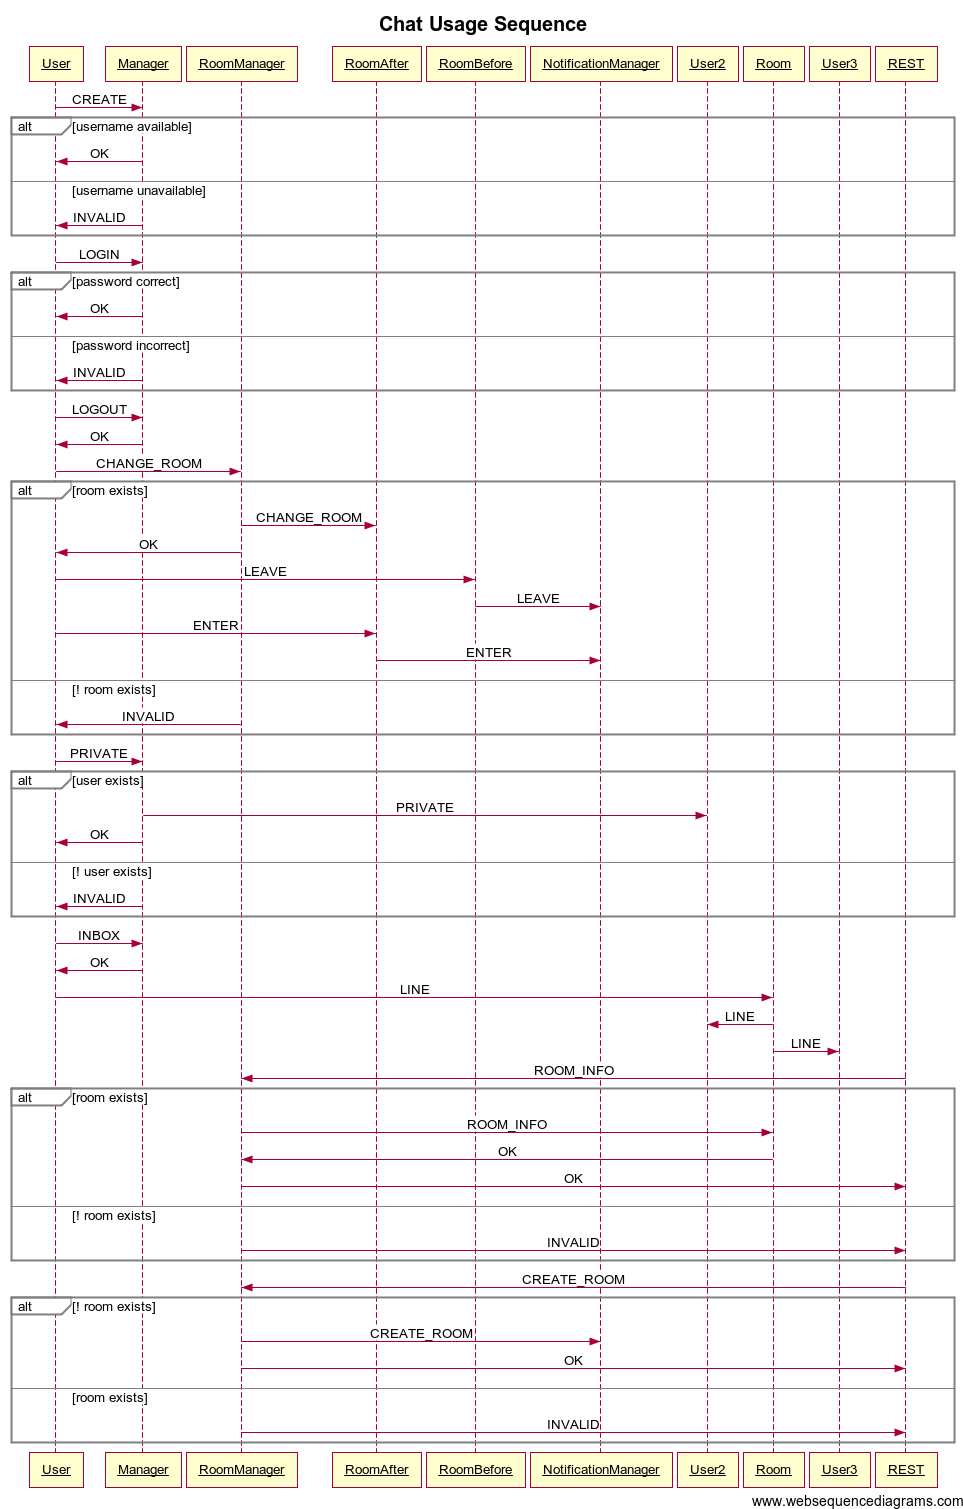
\includegraphics[width=1\textwidth]{seqdiag.png}
\caption{Sequence Diagram of Chat Usage}
\label{fig:seq_diag}
\end{figure}



%
% Telnet User
\subsection{User text protocol}

\begin{itemize}
\item cahsoicahscoiasc
\item :h/:help/:? - Lists all available commands\\
\item :cr/change new\_room - Change room\\
\item :logout - Logout \\
\item :login user pass - login to chat\\
\item :listrooms - Lists rooms\\
\item :listusers - Lists all users\\
\end{itemize}

%
% Rooms
\subsection{Chat rooms}


\section{Results}
\label{sec:results}
The first thing a user sees after connection to our system is the Authentication page.
    
The user has the option to log in, but only after creating an account. He can also remove an existing account. The system catches all this misuse alternatives and helps the user to the right path.

After the user is logged in, it is automatically in a chat room, the Main room, which is the default room of the service. In the simple text-based client, the user can type \emph{:help} to see the available commands. The GUI client has a panel that emulates just that: a text-box to write chat messages; a text area where the chat messages show up; a list of existing rooms or online users in a room; a button to go to his inbox; and, if it is an admin user, a button to go to admin options.

If the users clicks in the inbox, it can view the history of previous conversations with other users (:inbox command for the simple client lists only messages received) or send a private message to a user it never did before (:private user message for the simple client).

If an admin user clicks on the admin button option, it finds a panel where he can add or delete a room and give or take admin privileges to other users. 

In summary, all predictable error behaviour by the user is supported and information is displayed. During the implementation, other possible bugs were tested and, the ones found, were corrected.

Ex of a use situation and what happens when crashes and stuff



%
% Conclusions and Future Work
%



\section{Conclusions and Future Work}
\label{sec:conclusion}
This project was successful in emulating a Chat service comprising both a server and a client.

The project also has many features that make it scalable and easily maintainable. One issue that prevented the project to be more manageable was the way messages are in Quasar. They're not as flexible as, e.g., Erlang messages, in which we're not limited to the number of elements of the message neither their type.

Despite the fact that no major bugs were found, there is still room for improvement. 
Some tests should be developed to ensure that the system is running properly, to verify database performance and the communication between the GUI client and the server never fails. We think that a major improvement would be integrate the Notification Client in the Chat Client.

In conclusion, all the goal were meet and some further improvements were implemented. Therefore, we consider this a successful demonstration of a Chat Server.




%
% Bibliography
%

\bibliography{texinputs/bib}{}
\bibliographystyle{plain}


\appendix

\pagebreak

\section{API REST}
\label{app:rest}

\begin{table}[H]
\centering
\begin{tabular}{l|l}
\textbf{Endpoint} & \textbf{/rooms}\\
\hline
\textbf{HTPP method} & \textbf{GET}\\
\hline
\textbf{Response Codes} & 
 \begin{tabular}{l|l}
 200 & OK
 \end{tabular}
 \\
\hline
\textbf{Response} & \{"rooms":["Main, ShareLatex, Erlang"]\}\\
\hline

\end{tabular}
\caption{List rooms}
\end{table}

\begin{table}[H]
\centering
\begin{tabular}{l|l}
\hline
\textbf{Endpoint} & \textbf{/room/\{name\}}\\
\hline
\textbf{Parameters} & name - name of the room \\
\hline
\textbf{HTPP method} & \textbf{GET}\\
\hline
\textbf{Response Codes} & 
 \begin{tabular}{l|l}
 200 & OK \\
 404 & If the room does not exist
 \end{tabular}
 \\
\hline
\textbf{Response} & \{"name":"Main","users":["ana", "vitor"]\}\\
\hline

\end{tabular}
\caption{List users in room}
\end{table}


\begin{table}[H]
\centering
\begin{tabular}{l|l}
\hline
\textbf{Endpoint} & \textbf{/room/\{name\}}\\
\hline
\textbf{Parameters} & name - name of the room \\
\hline
\textbf{Headers} & \textbf{Volatile-ChatServer-Auth} - authentication \\
\hline
\textbf{HTPP method} & \textbf{PUT}\\
\hline
\textbf{Response Codes} & 
 \begin{tabular}{l|l}
 201 & Created \\
 401 & Unauthorized \\
 409 & If the room already exits \\
 \end{tabular}
 \\
\hline
\end{tabular}
\caption{Create room}
\end{table}

\begin{table}[H]
\centering
\begin{tabular}{l|l}
\hline
\textbf{Endpoint} & \textbf{/room/\{name\}}\\
\hline
\textbf{Parameters} & name - name of the room \\
\hline
\textbf{Headers} & \textbf{Volatile-ChatServer-Auth} - authentication \\
\hline
\textbf{HTPP method} & \textbf{DELETE}\\
\hline
\textbf{Response Codes} & 
 \begin{tabular}{l|l}
 200 & OK \\
 401 & Unauthorized \\
 404 & If the room does not exist \\
 412 & If the room still has users \\
 \end{tabular}
 \\
\hline
\end{tabular}
\caption{Delete room}
\end{table}


\begin{table}[H]
\centering
\begin{tabular}{l|l}
\textbf{Endpoint} & \textbf{/admin/\{username\}}\\
\hline
\textbf{Parameters} & username - username of the user \\
\hline
\textbf{Headers} & \textbf{Volatile-ChatServer-Auth} - authentication \\
\hline
\textbf{HTPP method} & \textbf{PUT}\\
\hline
\textbf{Response Codes} & 
 \begin{tabular}{l|l}
 201 & Created \\
 401 & Unauthorized \\
 404 & If the user does not exist 
 \end{tabular}
\hline
\end{tabular}
\caption{Make admin}
\end{table}

\begin{table}[H]
\centering
\begin{tabular}{l|l}
\hline
\textbf{Endpoint} & \textbf{/admin/\{username\}}\\
\hline
\textbf{Parameters} &  username - username of the user \\
\hline
\textbf{Headers} & \textbf{Volatile-ChatServer-Auth} - authentication \\
\hline
\textbf{HTPP method} & \textbf{DELETE}\\
\hline
\textbf{Response Codes} & 
 \begin{tabular}{l|l}
 200 & OK \\
 401 & Unauthorized \\
 404 & If the admin does not exists \\
 \end{tabular}
 \\
\hline
\end{tabular}
\caption{Detailed REST API.}
\end{table}



\section{OrientDB} 
\label{app:orientdb}


\subsubsection{Vertices}
\begin{itemize}
\item User: username, password, registrationDate, loggedIn, active;\\
\item Room: name, creationDate, active;\\
\item Message: from, to, text, date.
\end{itemize}


\subsubsection{Edges}
\begin{itemize}
\item Messages: from Room to Message: A room has all messages sent in that room linked with an edge; We're not linking the message to the user who sent it because there's no use for that now.\\
\item PrivateMessages: from User who sends to Message and from Message to User who receives: User's incomings edges are messages received; User's outgoing edges are messages sent.\\
\end{itemize}


\begin{figure}
\centering
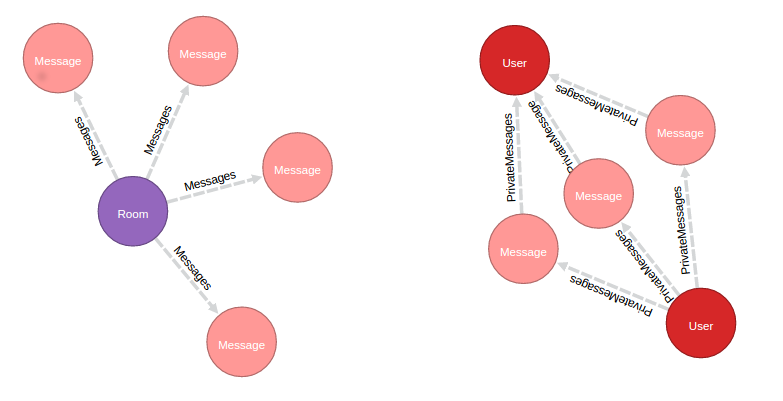
\includegraphics[width=\textwidth]{img/odb_graph.png}
\caption{OrientDB graph example.}
\label{fig:odbgraph}
\end{figure}



\end{document}

